\documentclass[report.tex]{subfiles}
\begin{document}

\chapter{Related Work} % (fold)
\label{cha:related_work}

% ==============================================================================
% ==============================================================================

\section{Non-Local Boxes} % (fold)
\label{sec:related_nlbs}
Non-local boxes (NLBs) are theoretical objects where multiple parties share some
correlation. The study of non-local boxes was introduced by physicists Sandu
Popescu and Daniel Rohrlich as part of their research on quantum non-locality.

Consider a device with two ends, held by Alice and Bob. Each provides an
input (\(x\) and \(y)\), and observe the output produced by the box (\(a\) and
\(b)\). The box is defined by the probability distribution \(P(a,b | x,y)\) 
where \(a, b, x, y \in {0, 1}\) \cite{nlb_lamontagne}. 

\begin{figure}[H]
  \centering
  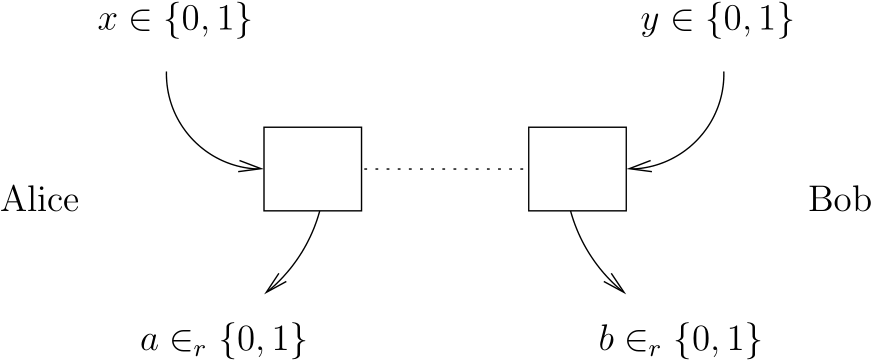
\includegraphics[width=0.66\textwidth]{img/nlb}
  \caption{A non local box \cite[Section~I]{2006quant.ph..9166D}}
\end{figure}

This device will immediately produce an output when given an input, preventing
any communication as a result of a delayed input. These devices are
non-signalling, ensuring that Alice cannot get any information about Bob's input
from her output, forbidding faster than light communication.

Popescu and Rohrlich introduced the concept of a non-local box a correlation 
that could achieve the algebraic maximum violation of 4 in the CHSH inequality
while also non-signalling \cite{ref1}, the CHSH inequality introduced by Clauser
et al being a constraint in quantum theory \cite{PhysRevLett.23.880}. This work
led to the further study of other non-local boxes as well, with expanded scope
in terms of the inputs and outputs of these boxes.
% subsubsection pr_box (end)

\subsection{Non-signalling} % (fold)
\label{sub:non_signalling}
As mentioned in Section \ref{sec:related_nlbs}, an important part of the
non-local box is that it is non-signalling. Non-signalling means that in the
described experiment, Alice cannot be made aware of Bob's choice of input or
vice-versa. This requirement imposes restrictions on the probability
distribution, since the probability of an output should depend solely on its
respective input. 

The non-signalling restriction can be represented by the given formulae
\cite[Section~II.A]{PhysRevA.71.022101}:
\begin{equation} \label{eq:non-signal_1}
\sum_{b} P(a, b | x, y) = \sum_{b} P(a, b | x, y') = P(a | x) 
\quad \forall a, x, y, y'
\end{equation}

\begin{equation} \label{eq:non-signal_2}
\sum_{a} P(a, b | x, y) = \sum_{a} P(a, b | x', y) = P(b | y) 
\quad \forall b, x, x', y
\end{equation}

These restrictions allow for a definition of a reduced probability on the
outputs as well, \(P(a | x)\), which is useful information to have when
working with non-local boxes. For example, the modelling of NLBs in PRISM relies
heavily on having a definition of reduced probabilities, meaning that the lack
of such information would impede on the creation of such models.
% subsection non_signalling (end)

\subsection{Example NLBs} % (fold)
\label{sub:example_nlbs}
Provided are some examples of standard non-local boxes. It is possible to have
non-local boxes with more than two inputs and outputs, and it is also possible
to have non-local boxes that handle a larger set of values than binary digits
as well. Note that for the tables below, the rows indicate input and the columns
indicate output.

\subsubsection{Classical Model} % (fold)
\label{ssub:classical_model}
The classical model is a simple example of a non-local box. In our theoretical
device, a coin is toss inside the device, and whatever result it gives is sent
as the output to Alice or Bob. This behaviour produces the following probability
distribution.

\begin{table}[H]
  \centering
  \begin{tabular}{l | c c c c}
      & 00 & 01 & 10 & 11 \\
      \hline
      00 & \(\frac{1}{2}\) & 0 & 0 & \(\frac{1}{2}\) \\
      01 & \(\frac{1}{2}\) & 0 & 0 & \(\frac{1}{2}\) \\
      10 & \(\frac{1}{2}\) & 0 & 0 & \(\frac{1}{2}\) \\
      11 & \(\frac{1}{2}\) & 0 & 0 & \(\frac{1}{2}\) \\
  \end{tabular}
  \caption{Probability Distribution}
  \label{tab:classical}
\end{table}

As you can see, this upholds the non-signalling requirement, since the
distribution shows that a change of one input cannot influence the output at the
other end of the device. 
% subsubsection classical_model (end)

\subsubsection{PR-Box} % (fold)
\label{ssub:pr_box}
The PR-box, originally proposed by and named after Popescu and Rohrlich, can be
considered the `Hello World' of non-local boxes. It is the most basic structure,
with two inputs and two outputs, and is the basis for this area of research.

The PR-Box has the following probability distribution:
\[
    P(a, b | x, y) = 
    \begin{cases}
        \frac{1}{2} & \quad a \text{ XOR } B = x \text{ AND } y \\
        0 & \quad \text{otherwise} \\
    \end{cases}
\]

This set-up can again be described using a matrix denoting the probabilities as
in \ref{ssub:classical_model}, although the above notation is commonly used in
papers related to quantum non-locality.

\begin{table}[H]
  \centering
\begin{tabular}{l | c c c c}
  & 00 & 01 & 10 & 11 \\
  \hline
  00 & \(\frac{1}{2}\) & 0 & 0 & \(\frac{1}{2}\) \\
  01 & \(\frac{1}{2}\) & 0 & 0 & \(\frac{1}{2}\) \\
  10 & \(\frac{1}{2}\) & 0 & 0 & \(\frac{1}{2}\) \\
  11 & 0 & \(\frac{1}{2}\) & \(\frac{1}{2}\) & 0 \\
\end{tabular}
  \caption{Probability Distribution}
  \label{tab:pr}
\end{table}
% subsection example_nlbs (end)
% section related_nlbs (end)

% ==============================================================================

\section{PRISM} % (fold)
\label{sec:prism}
PRISM \cite{KNP11} is a probabilistic model checking tool. It allows for
the modelling of systems which exhibit some random nature to them. Examples
include quantum cryptography or wireless networking protocols. Models as such
discrete-time Markov Chains can be created using the PRISM language, and
experiments can be ran using these models. Section \ref{sub:nlbs_in_prism}
provides an example of a non-local box in PRISM, breaking down the modules and
providing commentary on how it works.

PRISM uses a state based language, and includes tools for performing various
forms of analysis on a given model. A typical PRISM file will be made up of
multiple modules and variables, which interact with each other in various ways.
A module can read the values of other variables to update its own variables,
thus changing the state of the model. In addition, these modules can perform
synchronized actions with each other as well, meaning that multiple variables
can update in different modules simultaneously.

\subsection{NLBs in PRISM} % (fold)
\label{sub:nlbs_in_prism}
PRISM can be used for modelling non-local boxes, although it's weaknesses in 
doing so are the inspiration for this project. The PR-box described in
Section \ref{ssub:pr_box} will be used as the example model, which will be
broken down for easier understanding.

The box is represented using a discrete-time Markov Chain, meaning that the 
model will transition from one state to the next based only on the current
state, with no memory of the steps preceding.

\subsubsection{Input} % (fold)
\label{ssub:input}
\lstinputlisting[numbers = left, firstnumber = 1, linerange={3-9},
basicstyle=\ttfamily\footnotesize, frame=single,
caption={pr.qgrady input module.}, label={lst:inputmodule}]{files/pr.prism} 

Each input of the box is given its own module in the model. These modules
contain the variable that represents its input, initialised at -1 to indicate
that it's value is yet to be determined. Line 3 includes a guard indicating that
its actions can only be taken if \texttt{x} is equal to -1. In this case, it has
a 50/50 chance of being 0 or 1, effectively a coin toss.

Lines 5 and 6 provide a way to synchronize depending on the value of \texttt{x},
this is how the output module of the model will be alerted of the input's value,
and can then determine the appropriate output. As you can see, this does not
change the value of \texttt{x}, which will remain the same no matter what,
avoiding the potential for unwanted side effects.
% subsubsection input (end)

\subsubsection{Output Declaration} % (fold)
\label{ssub:output_declaration}
\lstinputlisting[numbers=left, firstnumber=1, linerange={19-27, 51},
basicstyle=\ttfamily\footnotesize, frame=single,
caption={pr.qgrady output module variables and synchronize flags.}
label={list:outputmodule}]{files/pr.prism} 

The output module includes all outputs produced by the box, with the addition of
a \texttt{ready} variable that acts as a block as part of the module. This has
the purpose of ensuring that when the module synchronizes with an input, the
respective output must be determined next before continuing. 

The output variables have similar synchronized actions that can allow parties 
interested in using the value of the output in determining the next state to
transition to.
% subsubsection output_declaration (end)

\subsubsection{Output Reduced Probabilities} % (fold)
\label{ssub:output_reduced_probabilities}
\lstinputlisting[numbers=left, firstnumber= 1, linerange={29-32},
basicstyle=\ttfamily\footnotesize, breaklines=true, frame=single, 
caption={Reduced probability of outputs.}, label={lst:reducedprob}]
{files/pr.prism} 

Moving onto the reduced probabilities. This is one reason why non-signalling
must be cared about. Its ability to provide a definition of the reduced
probabilities means that we can them as part of the model. In this instance,
each variable has a reduced probability of 50\% to be either 0 or 1. 

Note that the module must be ready in order to perform this action, synchronized
with the input actions acting as a flag alerting that this assignment can take
place.
% subsubsection output_reduced_probabilities (end)

\subsubsection{Output Normalised Probabilities} % (fold)
\label{ssub:output_normalised_probabilities}
\lstinputlisting[numbers=left, firstnumber= 1, linerange={34-41},
basicstyle=\ttfamily\footnotesize, breaklines=true, frame=single,
caption={Reduced probability of outputs.}, label={lst:normalisedprobs}]
{files/pr.prism} 

Finally, the normalised probabilities are considered. These actions take
advantage of knowing the existing values of the other input and output to
normalise the probabilities of the remaining output. For example, line 8 shows
that \texttt{y} equal to 1 and \texttt{b} equal to 1 shows that \texttt{a} can
only be 0 since the action is synchronizing with \texttt{x0}. The probabilities
in \ref{tab:pr} must have the now impossible outcomes ignored so that the
normalised probabilities can be determined for use in the model.
% subsubsection output_normalised_probabilities (end)

% subsection nlbs_in_prism (end)
% section prism (end)
% chapter related_work (end)

\newpage
\end{document}